\documentclass[a4paper,12pt]{article}
\usepackage[french]{babel}
\usepackage{amsfonts}
\usepackage{amsmath,amssymb,amsthm}
\usepackage{latexsym}

\usepackage[margin=1.5cm]{geometry}

\usepackage{graphicx}

%%%%%
% variable to include comments or not in the compilation ; set to 1 to include
\def \draft {1}
%\def \draft {0}


% writing utilities

% comments and responses
%  -> use this comment to ask questions on what other wrote/answer questions with optional arguments (up to 4 answers)
\usepackage{xparse}
\usepackage{ifthen}
\DeclareDocumentCommand{\comment}{m o o o o}
{\ifthenelse{\draft=1}{
    \textcolor{red}{\textbf{C : }#1}
    \IfValueT{#2}{\textcolor{blue}{\textbf{A1 : }#2}}
    \IfValueT{#3}{\textcolor{ForestGreen}{\textbf{A2 : }#3}}
    \IfValueT{#4}{\textcolor{red!50!blue}{\textbf{A3 : }#4}}
    \IfValueT{#5}{\textcolor{Aquamarine}{\textbf{A4 : }#5}}
 }{}
}


% todo
\newcommand{\todo}[1]{
\ifthenelse{\draft=1}{\textcolor{red!50!blue}{\textbf{TODO : \textit{#1}}}}{}
}





\begin{document}



\title{
% title propositions
%Space matters
For a Systematic Sensitivity Analysis of Spatial Meta-parameters in Models of Simulation
}


\date{}

\maketitle

\section{Space does matter in simulation modeling}

generalities about simulation modeling of social facts and initial conditions

the choice of working (as an illustration) on Schelling segregation model 

\subsection{Literature review on why we believe space actually does matter}

Pourquoi est-ce qu'on pense que forme grille spatiale peut influencer Schelling ?

Spatio-temporal model of a social fact, so spatio-temporal patterns and dynamics are important. Spatial grid as an input variable whose impact on the model behaviour and output should be systematically tested while looking for general conclusions : e.g. effect of the size of the neighbourhood on the decision to move.

clementine \& marion already started to write something up on that topic

\subsection{With a simple Schelling model}

simple illustration based on Netlogo Segregation model (Florent)
For now on: one agent per cell, some cells cannot host agents, Moore neighbourhood. The idea is to illustrate how this simple variation in the population density of a cell (0 or 1) will impact their neighbourhood and therefore the probability to host blue or red agents.

\subsection{In reality...}

(if enough material) : what type of cities actually produced more / less segregation?
See if there is some empirical findings the link between the shape of a city and its capability to produce segregated residential patterns.

end of section : we got frustrated and wanted to systematically study the influence of initial spatial configuration on how models (here Schelling) does behave

this is why...


%%%%%%%%%%%%%%%
\section{Research framework}
%%%%%%%%%%%%%%%


%%%%%%%%%%%%%%%
\subsection{But in reality space is more complicated than basic Schelling model}

We want to consider the fact that there are different morphologies of cities (so different topological relations between 'neighbouring' cells) and various level of densities at the block$/$residential building level (so for the same definition of the scope of a neighbourhood, not the same number of agents nor the same potentiality to host a new agent).

we worked with Schelling model extended with heterogeneous cell capacities: find the references of previous work where spatial heterogeneity and densities have been studied.

basic description of the model that we use, of the parameters and behaviour of agents that we simulate and finally of the output indicators.

Our output indicators: the level of segregation at equilibrium. Global indicator and$/$or also Local Moran's (number of significant clusters)?

What we are interested in is how the relation between the input variables and the output indicators may vary according to the spatial grid we're using. Not sure we have to mention it here, but just as a reminder for us.

We have to be explicit about the relation between density and neighbourhood: if neighbourhood is describe as a number of agents, or by a particular spatial scope that we vary. In monocentric cities with highly populated cells, large neighbourhoods won't make a difference as most of the cells won't have the capacity to host migrants. Etc.

Of course, we have to define what we call an equilibrium: static, dynamic (agents are still moving as there are still some unhappy ones but the segregation patterns$/$ values are not evolving anymore $\rightarrow$ we fix this time scope as being $n$ time steps). 



%%%%%%%%%%%%%%%
\subsection{And studying influence of space requires appropriate tools}

(which is maybe why scholars tend not to do that : it's hard)
our research framework : many combinations of parameters and many urban forms, plus random components (asynchronous decision making by agents which requires to order the agents...) : OpenMole to the rescue! 


%%%%%%%%%%%%%%%
\subsection{Generation of various urban forms}

Juste's density generation model and comparison with Florent's categories : 
now everything is on stage for the results




%%%%%%%%%%%%%%%
\section{How space matters}

Again we have two points of analysis: the range and variability of segregation levels per city types that we obtained and how the shape of cities impact on the model behaviour, i.e. the relation between input and output variables.


%%%%%%%%%%%%%%%
\subsection{Shape of cities and segregation capability}

We can imagine a figure where we would have one example of city of each type and two sizes of neighbourhood scope for instance (everything else being equal), and we see the resulting distribution of green and blue agents at equilibrium.

Plus descriptive statistics (factor analysis? regression?)



%%%%%%%%%%%%%%%
\subsection{Systematic analysis}


\paragraph{Systematic Exploration}

The relation between these values and the value of the input parameters $\rightarrow$ phase diagram better than a regression analysis for instance as we suppose the relations are not continuous. We want to see if there are (and if yes, where in the parameter space) the ruptures and clusters of same behaviours.

z(x,y) en fonction des formes de grilles initiales, z étant l'indice de segregation (Moran global ou nombre de clusters significatifs obtenus avec un local moran?) et (x,y) nos inputs (proportion of similar people wanted and size of the neighbourhood) 



\paragraph{Comparing Phase Diagrams}

Problem: we have as many phase diagrams than we have spatial grids, so we cannot define the phases qualitatively. We need quantitative procedures.

Potential methods to explore: anisotropic spatial segregation index (number of clusters found and where in the parameter spaces? but may be weak...), earth Movers Distance (i.e. distance between probability distributions), comparison of transition matrices of the dynamic associated to the potential...
See also: http://mck.riks.nl/ to get some ideas.


\paragraph{Results}

Et on met le mod{\`e}le plus sioux avec toutes les réplications dans plein de configurations de villes d'une part : diagramme de phase par rapport aux meta-param{\`e}tres(=indicateurs de forme, dans un plan principal = 80\% variance expliqu{\'e}e) de la variabilit{\'e} des diagrammes de phase selon critères de comparaison quantitatifs par rapport à une r{\'e}f{\'e}rence.





%%%%%%%%%%%%%%%
\subsection{Application: the Sugarscape model}

To illustrate the generic nature of our methodology, we apply it here to an other model implying a spatialized distribution of resources for which agents compete: the ``Sugarscape'' model, introduced in~\cite{epstein1996growing}.

Basic parameters if the sugarscape model on which phase diagrams are computed are: agent population $N$, agent minimal ressource $s_{min}$ and agent maximal ressource $s_{max}$.


%%%%%%%%%%%%%%%
\begin{figure}
\centering
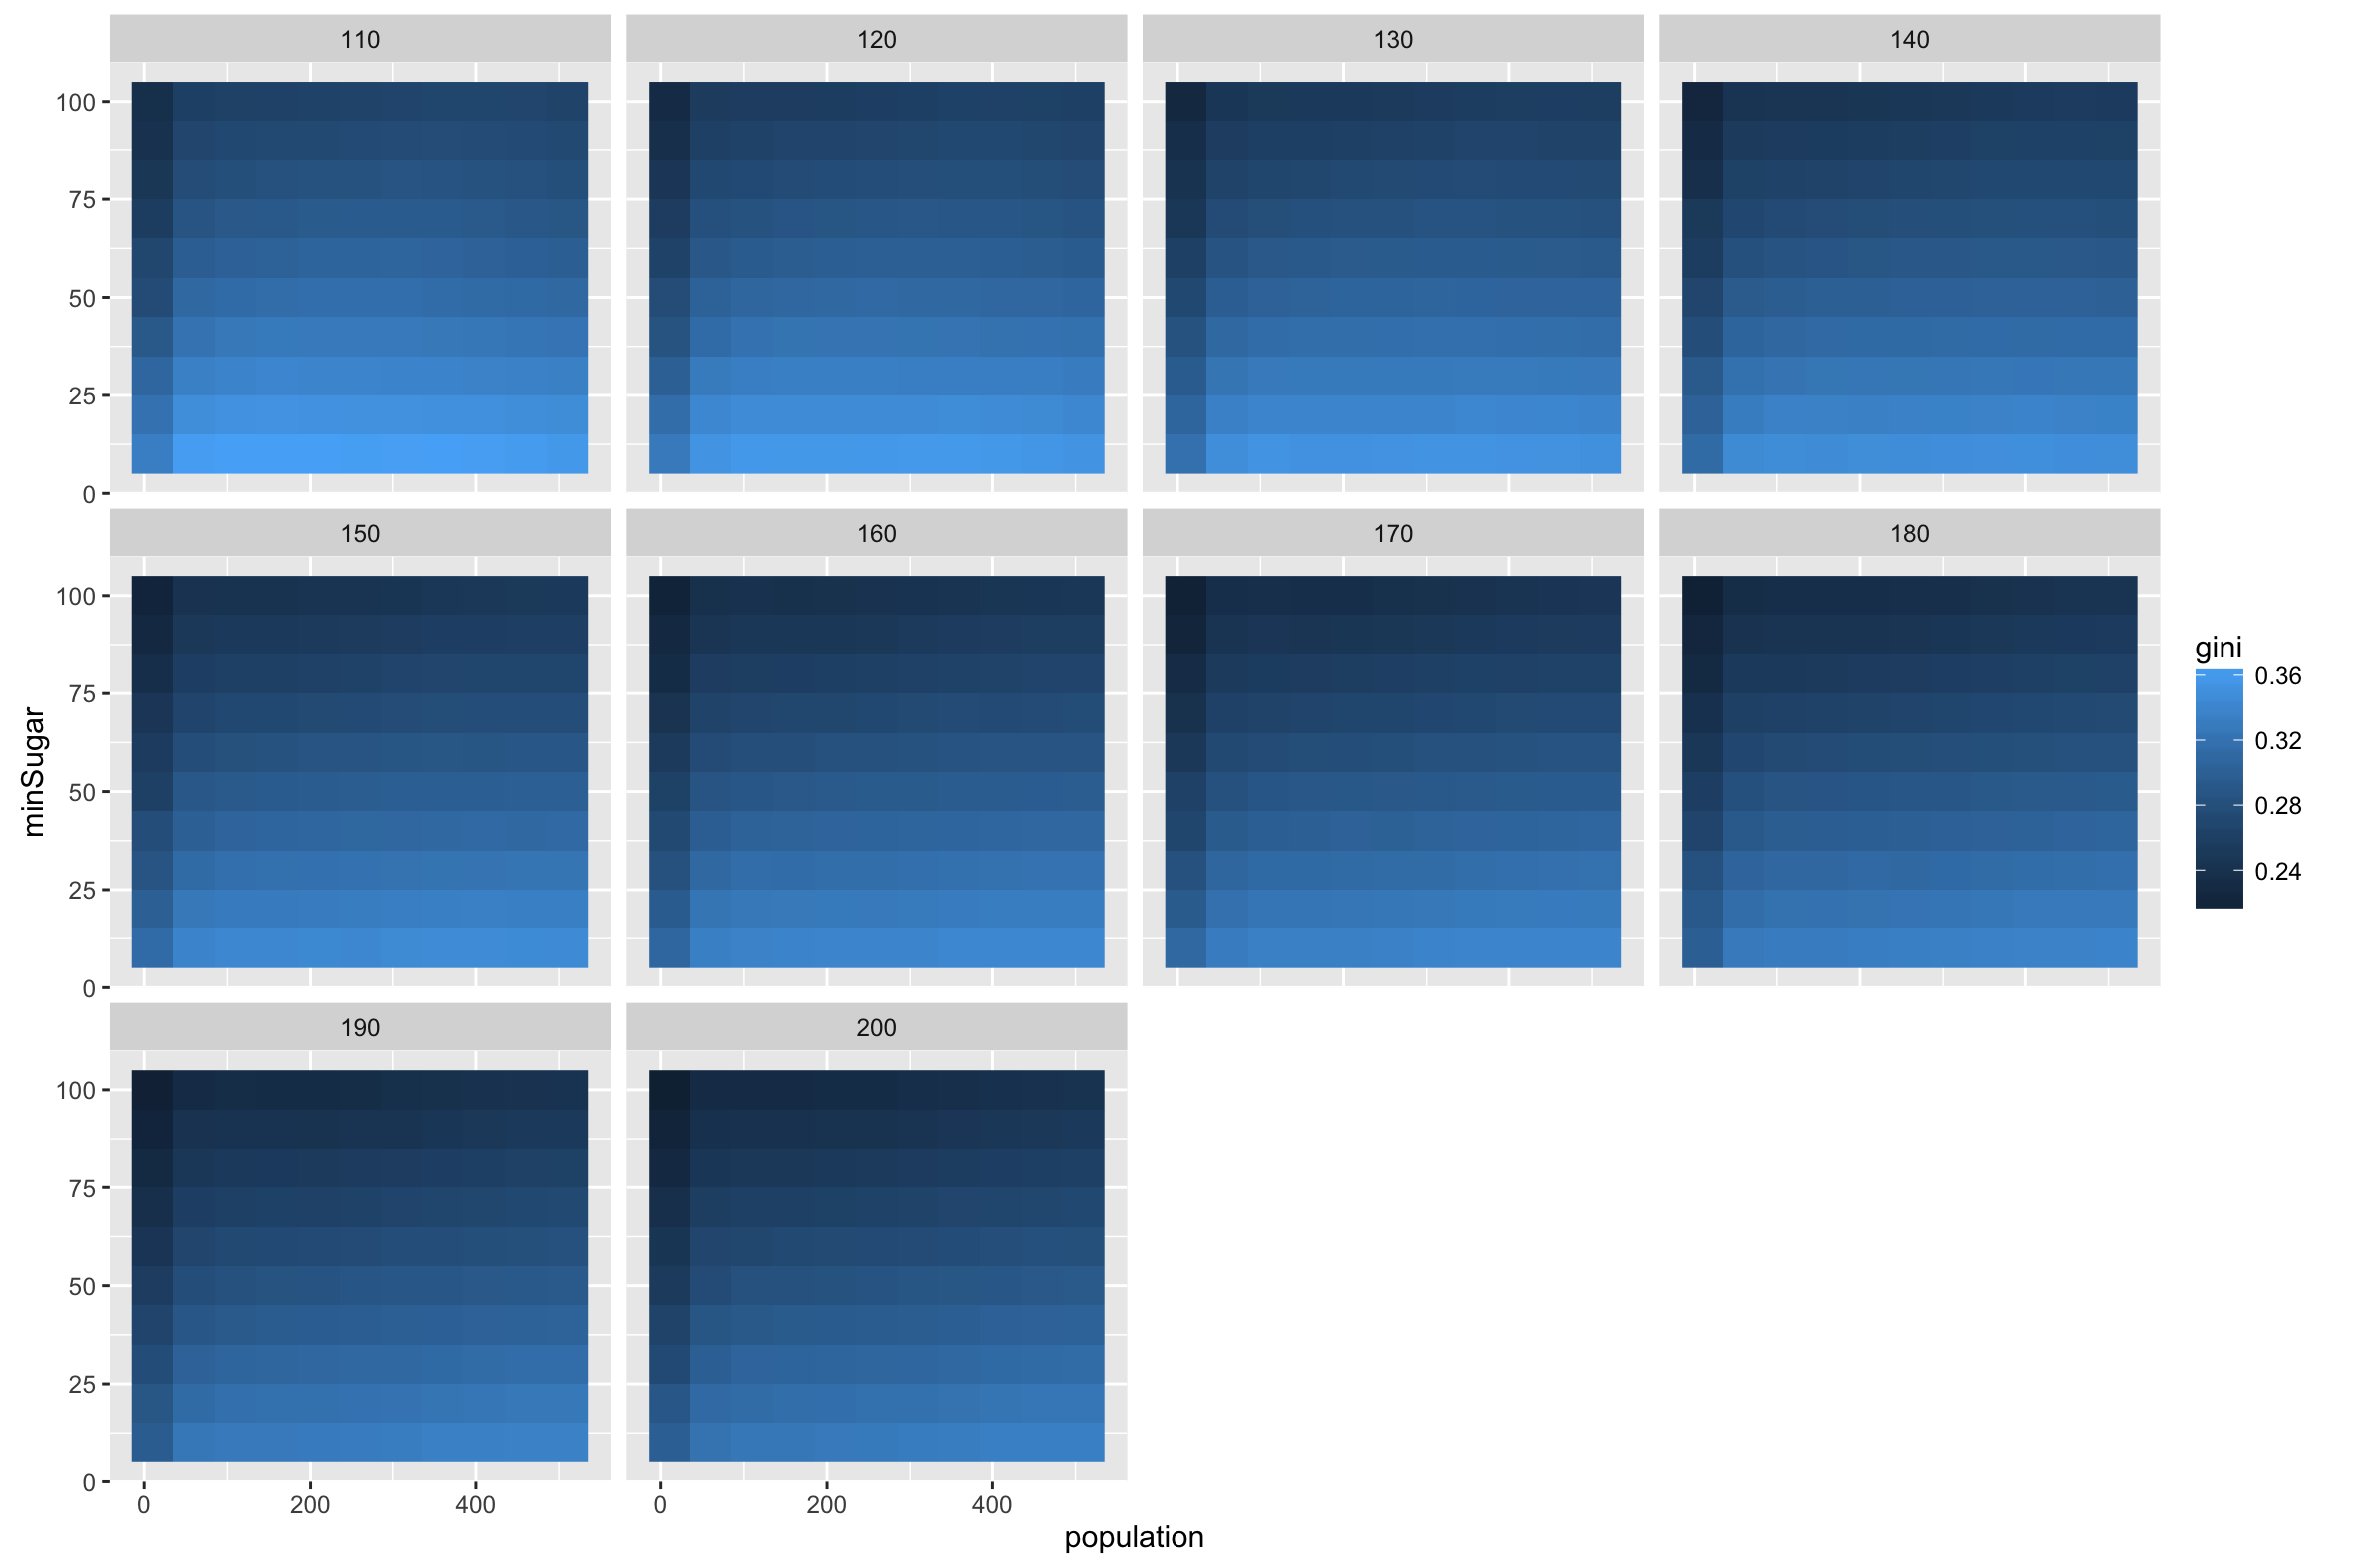
\includegraphics[width=\textwidth]{figures/fixed_phase_diagram}
\caption{Phase diagram of the sugarscape model (final smoothed Gini indicator), for a basic bicentric spatial setup, with varying parameters population $N$, minimal sugar reload $s_{min}$ and maximal sugar reload $s_{max}$. For each parameter point, average is taken over 50 repetitions.}
\label{fig:sugarscape-phasediagram}
\end{figure}
%%%%%%%%%%%%%%%


%%%%%%%%%%%%%%%
\begin{figure}
\centering
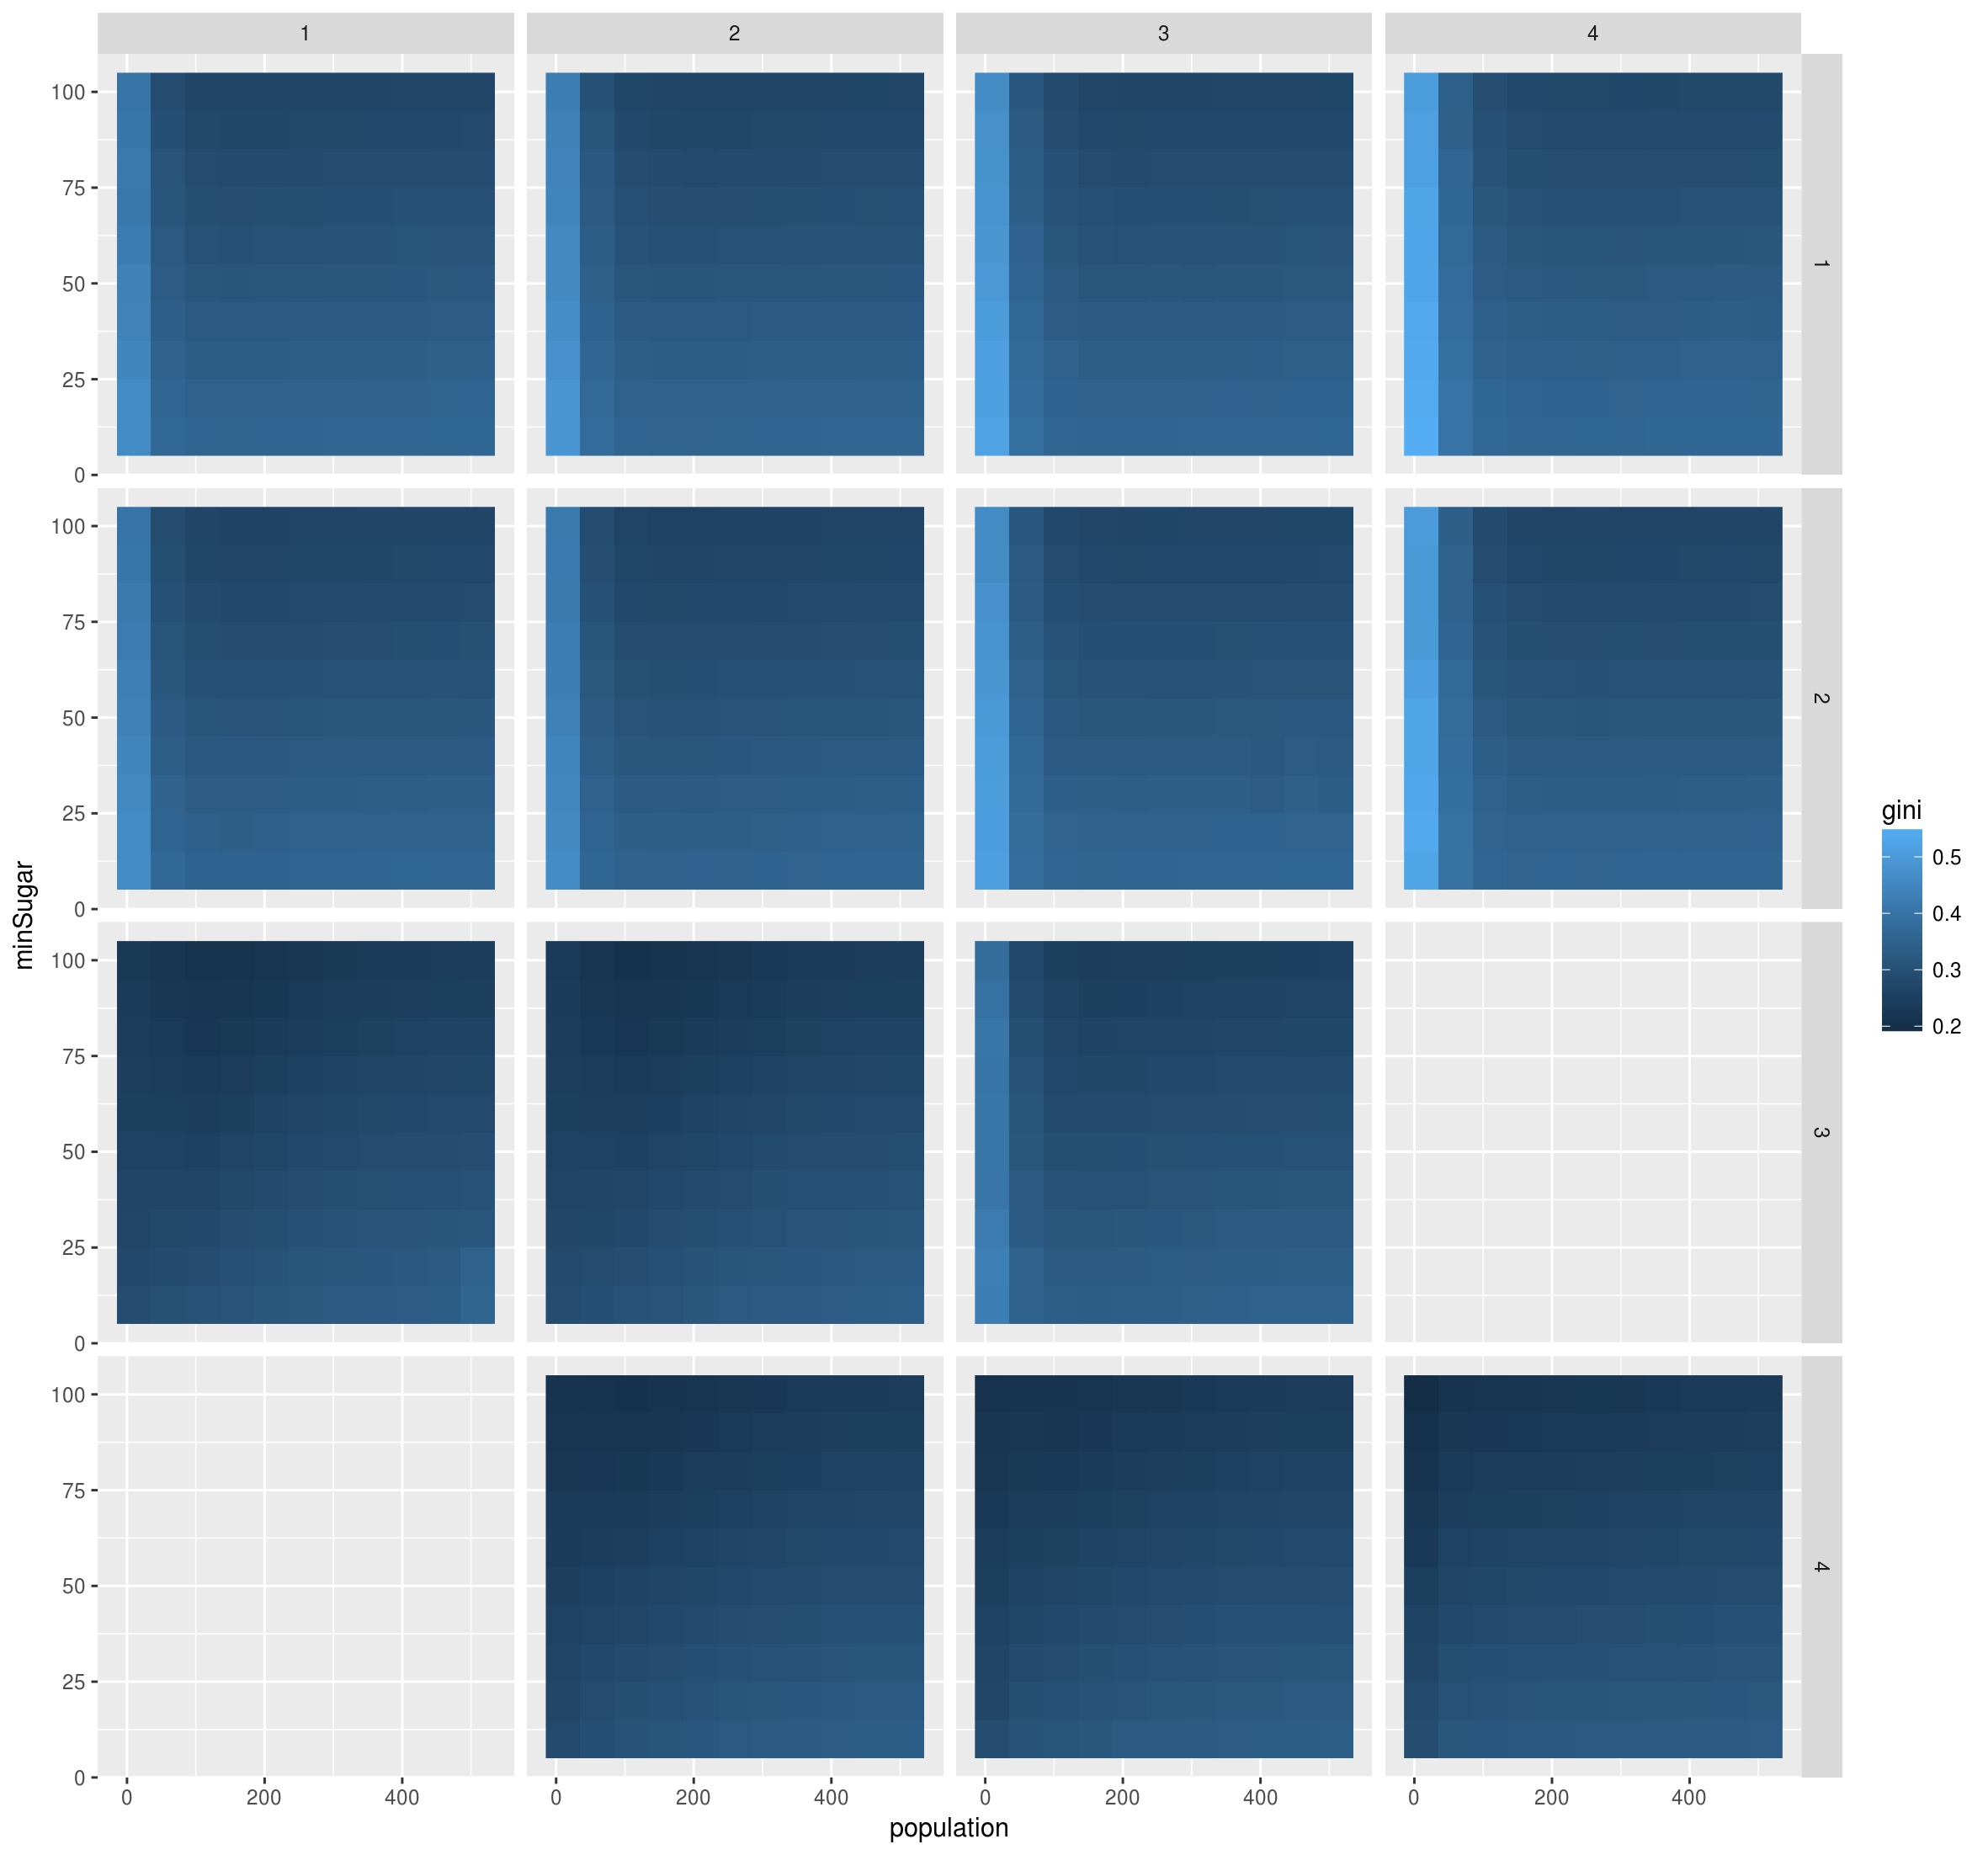
\includegraphics[width=\textwidth]{figures/phasediagrams_pca_maxSugar200}
\caption{Phase diagrams varying across the container morphological space. 50 realistic ressources distributions were generated, and used as container landscape (patches sugar capacity) for the sugarscape model, and phase diagrams were computed as in Fig.~\ref{fig:sugarscape-phasediagram} for each one. Spatial configurations were classified by reducing the dimension from four morphological indicators to two principal components ($\simeq$80\% of variance), for which the resulting space was gridded into 5x5 bins. We show here for each cell the average phase diagram along $(N,s_{min})$, taken at $s_{max}=200$. Other values of $s_{max}$ provide similar qualitative variations. The two missing cells correspond to non-feasible cells in the morphological space for the given generating model and parameters.}
\label{fig:sugarscape-meta}
\end{figure}
%%%%%%%%%%%%%%%

%%%%%%%%%%%%%%%
\begin{figure}
\centering
%
\caption{Meta phase diagram, i.e. phase diagram of phase diagram behavior, along parameters of spatial configuration generation ($\alpha$,$n_D$,$\beta$,$N_G$) (described these somewhere), aggregated for each as an Earth Mover Distance to a fixed reference (phase diagram of Fig.~\ref{fig:sugarscape-phasediagram}).}
\label{fig:sugarscape-meta}
\end{figure}
%%%%%%%%%%%%%%%


%%%%%%%%%%%%%%%
\subsection{Application: SimpopNet}

More complicated initial conditions such as a synthetic transportation network also fully enter our framework, even these may be more difficult to generate or explore. We illustrate this other type of application by exploring the sensitivity of the \emph{SimpopNet} model to the initial network. This model introduced in \cite{schmitt2014modelisation} aims at simulating the co-evolution of cities and transportation networks. The implementation of the model for which the behavior is known corresponds to a fixed stylized initial network. We modulate it here in a basic way, within a range of plausibility given by network indicators.








%%%%%%%%%%%%%%%
\section{Discussion}
%%%%%%%%%%%%%%%

Puis discussion : space matters (les valeurs prises par les indicateurs segrégations sont pas les mêmes) et ensuite en ouverture implications pour planning ?




%%%%%%%%%%%%%%%
% Biblio
%%%%%%%%%%%%%%%


\bibliographystyle{apalike}
\bibliography{biblio}






\end{document}